\documentclass[12pt,]{book}
\usepackage{lmodern}
\usepackage{amssymb,amsmath}
\usepackage{ifxetex,ifluatex}
\usepackage{fixltx2e} % provides \textsubscript
\ifnum 0\ifxetex 1\fi\ifluatex 1\fi=0 % if pdftex
  \usepackage[T1]{fontenc}
  \usepackage[utf8]{inputenc}
\else % if luatex or xelatex
  \ifxetex
    \usepackage{mathspec}
  \else
    \usepackage{fontspec}
  \fi
  \defaultfontfeatures{Ligatures=TeX,Scale=MatchLowercase}
    \setmonofont[Mapping=tex-ansi,Scale=0.7]{Source Code Pro}
\fi
% use upquote if available, for straight quotes in verbatim environments
\IfFileExists{upquote.sty}{\usepackage{upquote}}{}
% use microtype if available
\IfFileExists{microtype.sty}{%
\usepackage{microtype}
\UseMicrotypeSet[protrusion]{basicmath} % disable protrusion for tt fonts
}{}
\usepackage[margin=1in]{geometry}
\usepackage{hyperref}
\hypersetup{unicode=true,
            pdftitle={Mutational Genomics},
            pdfauthor={Dan MacLean},
            pdfborder={0 0 0},
            breaklinks=true}
\urlstyle{same}  % don't use monospace font for urls
\usepackage{natbib}
\bibliographystyle{apalike}
\usepackage{longtable,booktabs}
\usepackage{graphicx,grffile}
\makeatletter
\def\maxwidth{\ifdim\Gin@nat@width>\linewidth\linewidth\else\Gin@nat@width\fi}
\def\maxheight{\ifdim\Gin@nat@height>\textheight\textheight\else\Gin@nat@height\fi}
\makeatother
% Scale images if necessary, so that they will not overflow the page
% margins by default, and it is still possible to overwrite the defaults
% using explicit options in \includegraphics[width, height, ...]{}
\setkeys{Gin}{width=\maxwidth,height=\maxheight,keepaspectratio}
\IfFileExists{parskip.sty}{%
\usepackage{parskip}
}{% else
\setlength{\parindent}{0pt}
\setlength{\parskip}{6pt plus 2pt minus 1pt}
}
\setlength{\emergencystretch}{3em}  % prevent overfull lines
\providecommand{\tightlist}{%
  \setlength{\itemsep}{0pt}\setlength{\parskip}{0pt}}
\setcounter{secnumdepth}{5}
% Redefines (sub)paragraphs to behave more like sections
\ifx\paragraph\undefined\else
\let\oldparagraph\paragraph
\renewcommand{\paragraph}[1]{\oldparagraph{#1}\mbox{}}
\fi
\ifx\subparagraph\undefined\else
\let\oldsubparagraph\subparagraph
\renewcommand{\subparagraph}[1]{\oldsubparagraph{#1}\mbox{}}
\fi

%%% Use protect on footnotes to avoid problems with footnotes in titles
\let\rmarkdownfootnote\footnote%
\def\footnote{\protect\rmarkdownfootnote}

%%% Change title format to be more compact
\usepackage{titling}

% Create subtitle command for use in maketitle
\newcommand{\subtitle}[1]{
  \posttitle{
    \begin{center}\large#1\end{center}
    }
}

\setlength{\droptitle}{-2em}
  \title{Mutational Genomics}
  \pretitle{\vspace{\droptitle}\centering\huge}
  \posttitle{\par}
  \author{Dan MacLean}
  \preauthor{\centering\large\emph}
  \postauthor{\par}
  \predate{\centering\large\emph}
  \postdate{\par}
  \date{2017-05-19}

\usepackage{booktabs}
\usepackage{amsthm}
\makeatletter
\def\thm@space@setup{%
  \thm@preskip=8pt plus 2pt minus 4pt
  \thm@postskip=\thm@preskip
}
\makeatother
\setmainfont[UprightFeatures={SmallCapsFont=AlegreyaSC-Regular}]{Alegreya}
\renewcommand{\textfraction}{0.05}
\renewcommand{\topfraction}{0.8}
\renewcommand{\bottomfraction}{0.8}
\renewcommand{\floatpagefraction}{0.75}
\let\oldhref\href
\renewcommand{\href}[2]{#2\footnote{\url{#1}}}

\begin{document}
\maketitle

{
\setcounter{tocdepth}{1}
\tableofcontents
}
\listoffigures
\chapter*{Preface}\label{preface}
\addcontentsline{toc}{chapter}{Preface}

\section*{A fork is not a hairbrush - it just has some similar
properties}\label{a-fork-is-not-a-hairbrush---it-just-has-some-similar-properties}
\addcontentsline{toc}{section}{A fork is not a hairbrush - it just has
some similar properties}

Genomics has come a long way. We can now sequence genomes quickly and to
a reasonable degree of accuracy such that with sequence based approaches
we can create in a high-throughput manner an inventory of sub-regions in
a genome that we think are genes. We know the functions (or some of the
functions) of lots of genes and we can infer functions of newly
discovered genes by comparison of sequence or structure, basically by
seeing whether our new thing looks like something else.

But these methods are actually only PREDICTIONS of function. Looking a
bit like something else is only a clue to what something does. It
frequently fails us. We make the same mistake as Ariel in Figure
\ref{fig:ariel}.




\begin{figure}

\includegraphics[width=4.8in]{assets/ariel} \caption{Ariel thinks the fork is a brush, it does look like
one\ldots{}}\label{fig:ariel}
\end{figure}

\section*{So finding the function of a gene isn't
straightforward}\label{so-finding-the-function-of-a-gene-isnt-straightforward}
\addcontentsline{toc}{section}{So finding the function of a gene isn't
straightforward}

What makes things worse is that often we don't start with the gene
itself. We start with some biological process and want to find genes
with a role in that process. Because our functional predictions aren't
perfect we can't collect all the genes and start trying them out
one-by-one. It could take a while \ldots{} Figure \ref{fig:keys}.

\begin{figure}
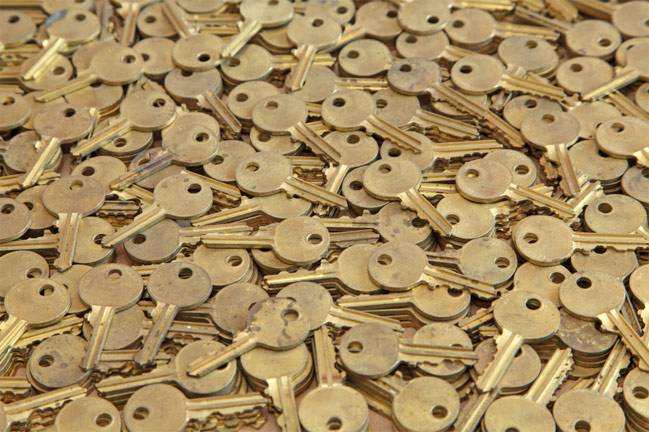
\includegraphics[width=4.33in]{assets/keys} \caption{One of these is the key to the bathroom. I hope that you're not desperate!}\label{fig:keys}
\end{figure}

\section*{We need something smarter - mutational genomics is this
smarter
thing}\label{we-need-something-smarter---mutational-genomics-is-this-smarter-thing}
\addcontentsline{toc}{section}{We need something smarter - mutational
genomics is this smarter thing}

With mutational genomics we deal initially with the effect of the gene
on the whole organism (Figure \ref{fig:mice} ). By performing
mutagenesis on our favourite organism then carrying out a screen that
selects individuals that have changed in the phenotype we are interested
in, we have our first foothold. We can study those individuals and apply
the principles of genetics, use modern high-throughput sequencing and
bioinformatics tools to identify the gene causing that phenotype change
(or at least ones involved in the process we have messed up).

\begin{figure}
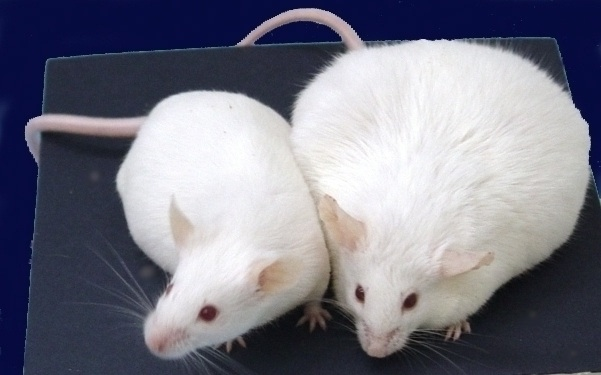
\includegraphics[width=4.01in]{assets/obese-mouse} \caption{One of these mice is not like the other mice - it has a phenotype change}\label{fig:mice}
\end{figure}

\section*{Our objective}\label{our-objective}
\addcontentsline{toc}{section}{Our objective}

This will be the focus of this workshop - how to go from samples
identified in a genetic screen to a short-list of candidate genes using
Galaxy tools and software.

\chapter{Mutagenesis}\label{mutagenesis}

\section{Learning Objectives}\label{learning-objectives}

\begin{itemize}
\tightlist
\item
  Mutagens make changes in a genome
\item
  EMS creates Single Nucleotide Polymorphisms of C-\textgreater{}T or
  G-\textgreater{}A Transition (mostly)
\item
  Careful crossing gives us homozygous mutant lines
\item
  Genetic screens select lines with changes related to our interest
\end{itemize}

\section{Mutagenesis with EMS}\label{mutagenesis-with-ems}

The first step is to mutagenise a population of organisms, or cells or
similar. Mutagenesis is basically causing damage to DNA. Lot's of things
can do this, Wikipedia has a great page on
\href{https://en.wikipedia.org/wiki/Mutagen}{mutagens}. In plant
genetics, the mutagen we typically use for changing single nucleotides
in DNA, things we call point mutations or Single Nucleotide
Polymorphisms (SNPs), is EMS -
\href{https://en.wikipedia.org/wiki/Ethyl_methanesulfonate}{Ethyl
methanesulfonate}. EMS will predominantly make C's change to T's and G's
change to A's. These mutations are distributed fairly uniformly
throughout the genome.

In practice we take a load of plant seeds and soak them in a solution of
EMS. The EMS soaks in and damages the plant's DNA.

This damages the DNA in \textbf{some} but \textbf{not all} of the cells
in the seed.

\section{Getting a population homozygous for EMS induced
mutations}\label{getting-a-population-homozygous-for-ems-induced-mutations}

We grow up the seed (let's call the plants that grow up the M1
generation) and the cells in those M1 plants that descended from the
mutagenised cells carry the mutations. Sometimes these will be cells in
the germline - ones that beget seeds. The progeny of the M1 plants, that
grow from mutation carrying seeds (let's call these progeny the M2) will
all grow up with the mutation \textbf{in every cell} and eventually, by
identifying the progeny plants carefully, we can get a population of
plants which are homozygous for all the EMS SNP mutations we induced.



\begin{figure}
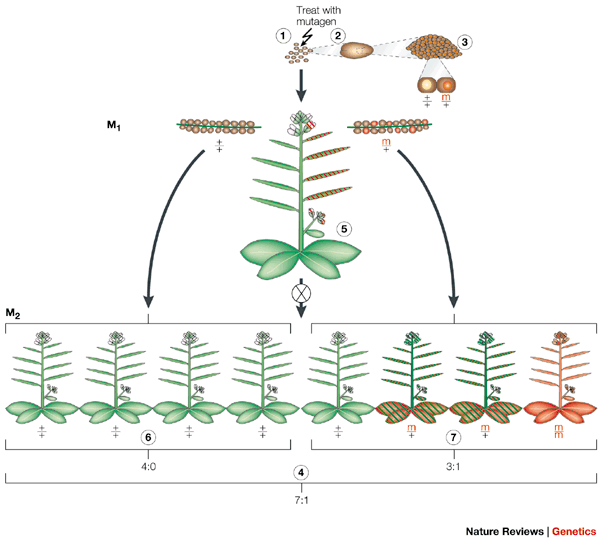
\includegraphics[width=4in]{assets/nrg730-i2} \caption{A plant mutagenesis scheme from \citet{Page:2002vm}.}\label{fig:mutagenesis}
\end{figure}

This same principle is true for any organism. Whatever you want to do
mutational genomics with, you will need to:

\begin{enumerate}
\def\labelenumi{\arabic{enumi}.}
\tightlist
\item
  mutate
\item
  select
\item
  cross
\item
  screen
\end{enumerate}

\section{Genetic screens}\label{genetic-screens}

Once we have a mutagenised population we can start to select the
individuals in that population that show some change in the phenotype of
interest, say flowering time. We can use further crosses to bring in
extra variation or use the natural variation - both of which are
heterozygous - while keeping the homozygous mutation(s) that is (are)
causing the phenotype by constantly selecting for offspring that show
the phenotype of interest everytime we carry out crosses.





\begin{figure}
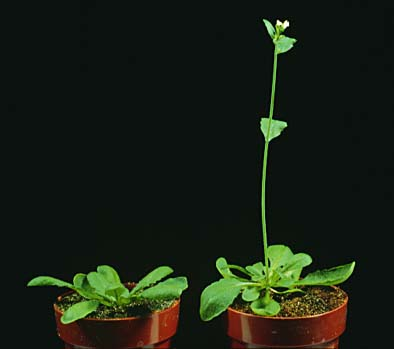
\includegraphics[width=5.47in]{assets/tall_plant} \caption{One of these plants is affected in the pathways that
control flowering time - the right hand plant flowers early. Source:
Detlef Weigel}\label{fig:tallplant}
\end{figure}

\section{Recombination during crossing causes changes in SNP density
away from the site of
mutation}\label{recombination-during-crossing-causes-changes-in-snp-density-away-from-the-site-of-mutation}

All these crosses cause recombination in the chromosomes that bring in
homologous parts from the line being used to cross. This happens at a
greater frequency away from the mutation that we are selecting for such
that regions further from the selected mutation carry fewer and fewer of
the homozygous mutations.






\begin{figure}
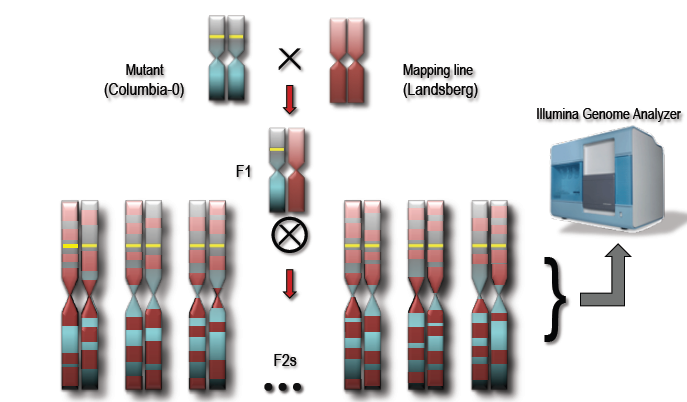
\includegraphics[width=4.58in]{assets/ngm} \caption{Consider crossing two chromosomes. Recombination causes
the parts furthest from the selected mutation to lose the homozygous
mutations as a function of distance from the selected mutation. Source:
\href{http://bar.utoronto.ca/ngm/description.html}{Ryan Austin}}\label{fig:ngm}
\end{figure}

This statistical difference, a region of high homozygous SNPs around the
mutation is what we will use to identify the SNPs that cause our
phenotype of interest.

\section{Section Quiz}\label{section-quiz}

Please now complete the section quiz at
\url{https://goo.gl/forms/RLGLndlcEcoV8c742}

\chapter{PreProcessing Data}\label{preprocessing-data}

\section{Learning Objectives}\label{learning-objectives-1}

\begin{itemize}
\tightlist
\item
  Understanding Fastq
\item
  Inspecting and interpreting the quality of sequence data with FASTQC
\item
  Cleaning out sequence data with trimmomatic.
\end{itemize}

\section{Fastq}\label{fastq}

\href{https://en.wikipedia.org/wiki/FASTQ_format}{Fastq} is a typical
sequence format generated by HTS machines. It contains four sections, a
sequence ID, the sequence, the ID again and a messy looking quality
string made up of characters, each of which represents the quality of
the base above it. Here's an example:

\begin{verbatim}
 @SEQ_ID
 GATTTGGGGTTCAAAGCAGTATCGATCAAATAGTAAATCCATTTGTTCAACTCACAGTTT
 +SEQ_ID
 !''*((((***+))%%%++)(%%%%).1***-+*''))**55CCF>>>>>>CCCCCCC65
\end{verbatim}

Each of the weird characters represents a number according to the
\href{https://en.wikipedia.org/wiki/ASCII}{\texttt{ASCII}} look up
table, where numbers are linked to characters, so \texttt{!} means
\texttt{33} and \texttt{"} means 34. These numbers are generally
\href{https://en.wikipedia.org/wiki/Phred_quality_score}{\texttt{Phred}}
scores, which encode the likelihood of the base being wrong on a log
scale.

We can use this quality information to assess how well our sequencing
went. Along with sequence quality information we should also assess the
composition of the sequence data. A program called FastQC \citep{FastQC}
is useful for this.

\subsection{Quality score encoding}\label{quality-score-encoding}

Different sequencers use slightly different variations on the Phred
score, this is usually called the quality encoding. Older Illumina
pipelines encoded a score from -5 to 62 using ASCII characters 59 to
126, but nowadays most use Sanger encoding, which encodes a score from 0
to 93 using ASCII 33 to 126.

Because of this discrepancy, it is necessary to sometimes be explicit
about the sequence encoding in Galaxy. We do this by setting the data
attributes of data files

\section{FastQC}\label{fastqc}

FastQC presents a range of plots and summary statistics, you need to
provide it with Fastq data.

A typical output like that in Figure \ref{fig:fastqc} shows the
\texttt{per\ base\ sequence\ quality}.





\begin{figure}
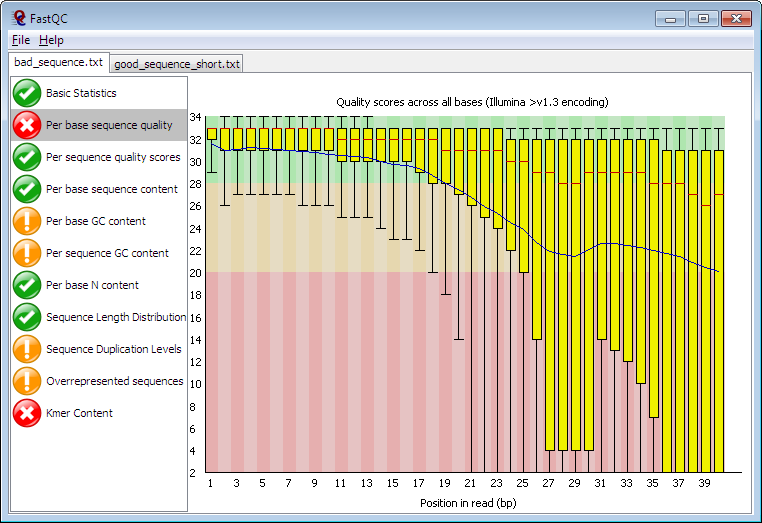
\includegraphics[width=5.08in]{assets/fastqc} \caption{FastQC Summary plot. Along the x-axis the plot shows
the position in the read and for each position in the reads it shows a
box-plot of all the quality scores at that position.}\label{fig:fastqc}
\end{figure}

The box plots to the left have much higher and tightly grouped quality
scores than those on the right. This is typical of Illumina machine
sequence, the quality decreases the further you get along the read. As
you can infer from the red region of the plot background, Phred scores
less than 20 are generally not trusted.

We may (or may not) decide that we need to get rid of the lower quality
sequence.

At the individual sequence read level, we can discard entire sequences
if part is too poor or trim the read leaving the good part alone. One
system for doing this is \citep{Bolger:2014ek} which can perform a
variety of trimming operations on sequence reads. It can remove parts of
reads from the left or right sides up to quality thresholds - it uses a
sliding window average, rather than just a harsh cut-off.

\subsection{Sometimes we shouldn't
trim}\label{sometimes-we-shouldnt-trim}

If we do carry out trimming, then we may end up with lots of reads of
different lengths - this can be a problem for some aligners and
downstream tools, so sometimes trimming isn't the best strategy, we have
to make context dependent decisions.

At the sequence sample level (e.g, the read file level), we may discover
that our read set is not good. Reports from FastQC like the \emph{k}-mer
content plot (Figure \ref{fig:kmer}) can show sequence problems, in this
graph there is an over-representation of particular \emph{k}-mers at the
start of the sequence that shouldn't be there.





\begin{figure}
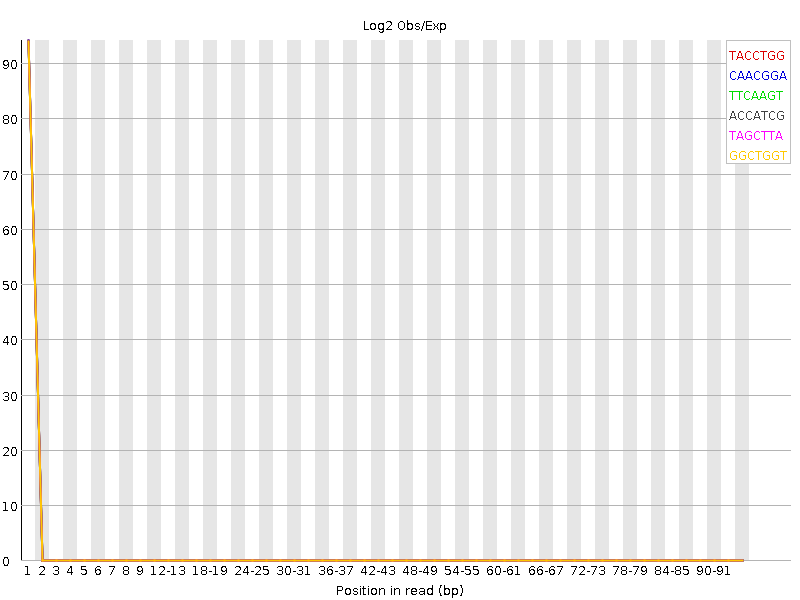
\includegraphics[width=5.33in]{assets/kmer_content} \caption{The first few bases here are significantly enriched, this
can be due to sequence adapters (if they were used) but if not, then the
sequence is likely not good, even if the quality scores are fine.}\label{fig:kmer}
\end{figure}

\section{Exercises}\label{exercises}

Your task now is to load up Galaxy and run some reads through quality
control and trimming, prior to downstream use.

\subsection{Power Up The VM}\label{power-up-the-vm}

\begin{enumerate}
\def\labelenumi{\arabic{enumi}.}
\tightlist
\item
  Start \texttt{VirtualBox} by double-clicking it's application icon.
\item
  Use \texttt{File} .. \texttt{Import\ Appliance} and select the
  \texttt{??????} VM file.
\end{enumerate}

\subsection{Start Galaxy}\label{start-galaxy}

Galaxy should appear ready and waiting in the Chromium browser on the
desktop in the VM. The bookmarks bar in this browser has all the links
you need for this workshop.

\subsection{Run FastQC}\label{run-fastqc}

Use the reads in the \texttt{Pre-processing} data library. You will find
the \texttt{FastQC} tool in the tool list under \texttt{HTS\ QC}. The
reads are single ended from mutagenised \emph{Arabidopsis thaliana}.
They are Illumina
\href{https://en.wikipedia.org/wiki/Shotgun_sequencing}{Whole Genome
Shotgun reads}, the sequence pipeline from our provider should have
removed any multiplex adapters and the plants are grown in sterile
culture so we aren't expecting contamination.

Please now complete the section quiz at
\url{https://goo.gl/forms/GBnZKO2Yt6hROAvw2}.

\begin{enumerate}
\def\labelenumi{\arabic{enumi}.}
\tightlist
\item
  How many reads are you using?
\item
  What sort of output files do you get from FastQC?
\item
  What should you do with these files?
\item
  Do they represent a scientific control that could be published?
\end{enumerate}

\hypertarget{qualprac}{\subsection{Interpret Sequence
Quality}\label{qualprac}}

\begin{enumerate}
\def\labelenumi{\arabic{enumi}.}
\tightlist
\item
  Is there any evidence of contamination? Which report tells you?
\item
  If there is, which sequence is contaminating?
\end{enumerate}

\subsection{Clean Up Poor Quality
Sequence}\label{clean-up-poor-quality-sequence}

Use the \texttt{Trimmomatic} tool in \texttt{HTS\ QC}.

\begin{enumerate}
\def\labelenumi{\arabic{enumi}.}
\tightlist
\item
  Find and try a trimming strategy to get rid of problems you observed
  in the section on \protect\hyperlink{qualprac}{interpreting sequence
  quality}. Select an appropriate \texttt{Average\ quality\ required}?
\item
  Which trimming strategy improves the set of reads?
\item
  How could you filter on size if you needed to pass only good quality,
  full length sequences to the next step?
\end{enumerate}

\chapter{Aligning Reads To A
Reference}\label{aligning-reads-to-a-reference}

\section{Learning Objectives}\label{learning-objectives-2}

\begin{itemize}
\tightlist
\item
  Understanding Alignment
\item
  Know how to run the correct BWA alignment
\item
  Understand the SAM/BAM format and relationship
\end{itemize}

\begin{quote}
Culture Clash

If you're a bioinformatician - you may be wondering why I'm not using
the words `mapping' reads here. Well, the geneticists in the crowd have
a much older technique called
\href{https://en.wikipedia.org/wiki/Gene_mapping}{mapping} that does
something completely different. I have honestly had conversations where
it has been insisted that I can't possibly map a read. Don't suffer as I
did.

If you're a geneticist - bioinformaticians claim they can do amazing
things with reads, mapping them down to the single read level! Of course
they usually just mean they're aligning them to whatever reference
sequence they have.
\end{quote}

\section{Mapping and Alignment}\label{mapping-and-alignment}

Mapping is the process of finding the position on a genome that a read
best matches to, so is likely to have come from. Alignment is the
optimal alignment of the sequence of the read with the reference
sequence, such that gaps and errors are allowed and small variations can
be found.

\subsection{BWA}\label{bwa}

There are many tools for aligning reads (too many, probably). One of the
best general ones is BWA \citep{Li:2010bl}. BWA is a high-throughput
sequence aligner used to align relatively short sequences to a reference
genome. It uses the Burrows-Wheeler Transform reduce the amount of
memory needed to align reads by creating a compressed index of the
reference sequence. It contains two algorithms for alignment, one
\texttt{aln} for short reads up to around 200 bp with low error rate and
another \texttt{mem} for longer reads. Both are very fast and accurate.

BWA is complicated and there are lots of options to set. The crucial
things we are going to need are a reference genome, and a set of reads.

Often, a sequencing strategy will use
\href{https://www.illumina.com/technology/next-generation-sequencing/paired-end-sequencing_assay.html}{paired-end
reads}, where we know the distance between two reads and we can set that
as a parameter. Usually the reads from a paired strategy come in two
files, one of the pair in a `left' file, and the other in a `right'
file.

BWA has a lot of options, here's some important ones:

\begin{enumerate}
\def\labelenumi{\arabic{enumi}.}
\tightlist
\item
  \texttt{Maximum\ edit\ distance} - is the maximum number of
  nucleotides in a read that can mis-match with the reference and the
  read still be aligned.
\item
  \texttt{Maximum\ number\ of\ gap\ opens}- refers to the amount of
  insertions that can occur across a read.
\item
  \texttt{Disallow\ insertion/deletion\ within\ some\ bp\ towards\ the\ end}
  - allows for the fact that sequence quality deteriorates towards the
  end of a sequence and the user might not want to trust indels in the
  last few bases of a read.
\item
  \texttt{Maximum\ insert\ size\ for\ a\ read\ pair\ to\ be\ considered\ as\ being\ mapped\ properly}
  - The insert size of reads is the distance between the outer ends of
  the two paired-end reads.
\end{enumerate}

\subsection{SAM Format}\label{sam-format}

The output format from BWA and most other aligners is
\href{https://en.wikipedia.org/wiki/SAM_(file_format)}{Sequence
Alignment Map} (SAM) format \citep{Li:2009ka}. The SAM format describes
the alignment of sequenced reads to a reference sequence. It stores all
the alignment information generated by BWA in a simple and compact
format. It provides information about the position of the read in
relation to the reference genome, the number and position of nucleotides
that match to the genome and the position of indels. SAM files are often
analysed in packages like SAMTools \citep{Li:2009ka} and Picard
(\href{https://broadinstitute.github.io/picard/}{Picard})

Here's the top of a SAM file:

\begin{verbatim}
@HD VN:1.3  SO:coordinate
@SQ SN:chloroplast  LN:154478
@PG ID:bwa  PN:bwa  VN:0.7.10-r876-dirty    CL:bwa mem -t 1 -v 1
chloroplast-1781    99  chloroplast 54  60  250M    =   374 570 TTA A?? NM:i:0  MD:Z:250    AS:i:250    XS:i:0
chloroplast-757 163 chloroplast 66  60  250M    =   459 643 GCT A5? NM:i:6  MD:Z:46A20T65T56A23A2T32    AS:i:220    XS:i:0
chloroplast-1781    147 chloroplast 374 60  250M    =   54  -570    ACT G:E NM:i:6  MD:Z:9T42G1G2G7C42A141  AS:i:220    XS:i:0
chloroplast-703 163 chloroplast 437 60  250M    =   794 607 AGC ??? NM:i:8  MD:Z:68T2C20C68T16G9A30A8G21    AS:i:210    XS:i:0
\end{verbatim}

\begin{enumerate}
\def\labelenumi{\arabic{enumi}.}
\tightlist
\item
  The first few lines start with stuff like \texttt{@SQ\ SN} which
  described thigs like program parameters followed by the name of the
  sequences in the reference file (\texttt{chloroplast}) and the length
  of the sequence (154478).
\item
  Every line after that corresponds to each read that BWA handled.
\item
  Each line starts with the name of the read and has a number of columns
  of data after it.
\item
  In the 3rd column we can see which chromosome our read has been mapped
  to and the position of the first mapped base in column 4. An unmapped
  read will have a * in column 3 and zero in column 4.
\item
  The 5th column is the mapping quality, a score quantifying the
  probability that a read is misplaced.
\item
  The 6th column is the CIGAR string and consists of numbers followed by
  an upper-case letter (the operator), which describes the alignment.
\end{enumerate}

As an example, a CIGAR string of \texttt{36M3D40M} means 36 matching
nucleotides, followed by 3 deletions and ending in 40 matches.

A BAM file is a highly compressed, indexed binary version of SAM and
through a library of different tools, allows fast, random access to the
alignment. Some Galaxy tools will automatically convert the output from
aligners to BAM format for you - (BWA does this!).

\section{Exercises}\label{exercises-1}

\subsection{Align Paired-End Reads To A Reference
Genome}\label{align-paired-end-reads-to-a-reference-genome}

Use the two sets of paired reads in the \texttt{Alignment} shared data
library and the \texttt{ATH1\_chloroplast} reference genome sequence, to
carry out a HTS alignment. Again these are sequences from the
chloroplast genome of the model plant \emph{Arabidopsis} . One set of
reads, \texttt{MS}, are from an Illumina MiSeq machine, are 250 nt long
and have a fragment length of 650 nt. The others, \texttt{GA2} are from
an Illumina GAII machine, are 75 nt long and have a fragment length of
350.

Please complete the section quiz at
\url{https://goo.gl/forms/l3ykUt7eNvZAM9Y42}

\begin{enumerate}
\def\labelenumi{\arabic{enumi}.}
\tightlist
\item
  Which algorithm should you use for each set of reads?
\item
  Align each of these with the BWA program in the
  \texttt{HTS\ Alignment} tools section. Choose an appropriate algorithm
  for each sequence set.
\item
  Pick parameters to make the two alignments as accurate and equivalent
  as possible? Which should differ? Which should be the same?
\item
  Check the results with the SAMtools \texttt{idxstats} tool and other
  alignment stats tools like \texttt{Flagstat} and \texttt{Stats} in
  \texttt{HTS\ SAMtools}. How do the results relate to what you know
  about the sequencing strategy? (What are the calculated insert sizes,
  what is the coverage, how many reads map?)
\end{enumerate}

\subsection{Merge Alignments Into One
BAM}\label{merge-alignments-into-one-bam}

After alignment of two read sets from different sequencing strategies,
you might want to merge all of them into one BAM file so that you can
work on them as one. This isn't just more convenient, it lets you make
use of the extra information from combining the reads into one coverage
pileup when calling SNPs or visualising the alignment.

Merging is a multi-stage process that can be done with
\href{https://broadinstitute.github.io/picard/}{Picard}, the steps in
Picard look like:

\begin{enumerate}
\def\labelenumi{\arabic{enumi}.}
\tightlist
\item
  Remove duplicate reads
\item
  Sort BAMs individually
\item
  Merge BAMs
\end{enumerate}

Picard tools are available in the \texttt{Picard} tool section. Try
merging the BAM files.

\subsection{Alignment Quality}\label{alignment-quality}

The \texttt{HTS\ SAMtools} tool \texttt{BAM-to-SAM} will allow you to
turn the binary BAM file into a SAM file you can read.

\begin{enumerate}
\def\labelenumi{\arabic{enumi}.}
\tightlist
\item
  How good do the individual alignments look overall? Can you tell from
  the output? Is it useful to look at single alignments one by one?
\item
  In what cases might the individual alignments be useful?
\end{enumerate}

\chapter{Finding SNPs With An
Alignment}\label{finding-snps-with-an-alignment}

\section{Learning Objectives}\label{learning-objectives-3}

\begin{itemize}
\tightlist
\item
  Understanding Pileups and VCFs
\item
  Calling reliable SNPs
\item
  Annotating SNPs with SNPEff
\end{itemize}

Many different programs can be used to call SNPs, including SAMTools
\citep{Li:2009ka}, Picard, GATK \citep{DeSumma:2017kr} and VarScan
\citep{Koboldt:2009dk}. Some of these programs use the BAM alignment
file directly, some use an MPileup file. MPileups and VCF files are both
used to represent SNPs and associated scores.

\section{MPileup}\label{mpileup}

The MPileup format is a per-line base-by-base representation of the
alignment. It provides a much more coherent way of viewing the alignment
than the SAM file.

Here's a sample:

\begin{verbatim}

seq1 272 T 24  ,.$.....,,.,.,...,,,.,..^+. <<<+;<<<<<<<<<<<=<;<;7<&
seq1 273 T 23  ,.....,,.,.,...,,,.,..A <<<;<<<<<<<<<3<=<<<;<<+
seq1 274 T 23  ,.$....,,.,.,...,,,.,...    7<7;<;<<<<<<<<<=<;<;<<6
seq1 275 A 23  ,$....,,.,.,...,,,.,...^l.  <+;9*<<<<<<<<<=<<:;<<<<
seq1 276 G 22  ...T,,.,.,...,,,.,....  33;+<<7=7<<7<&<<1;<<6<
seq1 277 T 22  ....,,.,.,.C.,,,.,..G.  +7<;<<<<<<<&<=<<:;<<&<
seq1 278 G 23  ....,,.,.,...,,,.,....^k.   %38*<<;<7<<7<=<<<;<<<<<
seq1 279 C 23  A..T,,.,.,...,,,.,..... ;75&<<<<<<<<<=<<<9<<:<<
\end{verbatim}

Each line represents a single nucleotide in the reference. The first
three columns represent the reference name, position on the reference
and the reference nucleotide.

The next three columns are about the bases piled-up over that position,
so are total read depth, read bases, and base qualities.

At the read base column,

\begin{itemize}
\tightlist
\item
  a dot \texttt{.} = a match to the reference base on the forward
\item
  a comma \texttt{,} = match on the reverse strand
\item
  any of \texttt{ACGTN} = a mismatch on the forward strand
\item
  any of \texttt{acgtn} = mismatch on the reverse strand
\end{itemize}

\subsection{Different Flavours of
PileUp}\label{different-flavours-of-pileup}

Pileup format has been extended at various times, so the exact format
you get can vary a little, the description above is the core of them all
and the extensions usually provide some further quality information.
Recent versions of SAMtools add quite a few columns to this description.

You can see more here \url{http://samtools.sourceforge.net/pileup.shtml}

\texttt{SAMtools} is usually used to generate an MPileup, the
\texttt{mpileup} command can do this. More recent versions of
\texttt{SAMtools\ mpileup} and most other SNP callers can also generate
another type of SNP describing file, a VCF
\href{https://samtools.github.io/hts-specs/VCFv4.2.pdf}{Variant Call
Format} file.

The related VCF file takes a slightly different approach and looks like
this:

\begin{verbatim}
##FORMAT=<ID=DP,Number=1,Type=Integer,Description="Read Depth">
##FORMAT=<ID=HQ,Number=2,Type=Integer,Description="Haplotype Quality">
#CHROM POS ID REF ALT QUAL FILTER INFO FORMAT NA00001 NA00002 NA00003
20 14370 rs6054257 G A 29 PASS NS=3;DP=14;AF=0.5;DB;H2 GT:GQ:DP:HQ 0|0:48:1:51,51 1|0:48:8:51,51 1/1:43:5:.,.
20 17330 . T A 3 q10 NS=3;DP=11;AF=0.017 GT:GQ:DP:HQ 0|0:49:3:58,50 0|1:3:5:65,3 0/0:41:3
20 1110696 rs6040355 A G,T 67 PASS NS=2;DP=10;AF=0.333,0.667;AA=T;DB GT:GQ:DP:HQ 1|2:21:6:23,27 2|1:2:0:18,2 2/2:35:4
20 1230237 . T . 47 PASS NS=3;DP=13;AA=T GT:GQ:DP:HQ 0|0:54:7:56,60 0|0:48:4:51,51 0/0:61:2
20 1234567 microsat1 GTC G,GTCT 50 PASS NS=3;DP=9;AA=G GT:GQ:DP 0/1:35:4 0/2:17:2 1/1:40:3
\end{verbatim}

The first thing you notice is that it describes only variant positions
\textbf{NOT} \textbf{EVERY} position like Pileup.

The lines starting with \texttt{\#\#} are the meta-data description
lines. They define the labels for SNP data and contain key-value pairs
separated by an `=' sign (e.g.~number=1, Type=Integer,
Description=``Some description'').

The header line starts with a single \texttt{\#}, and has the column
headings, these being \texttt{ALT} and \texttt{QUAL}.

\begin{enumerate}
\def\labelenumi{\arabic{enumi}.}
\tightlist
\item
  \texttt{CHROM} = chromosome
\item
  \texttt{POS} = position
\item
  \texttt{ID} = an ID (if given)
\item
  \texttt{REF} = reference sequence nucleotide
\item
  \texttt{ALT} = SNP nucleotide
\item
  \texttt{FILTER} = a filter defined in the metadata
\item
  \texttt{INFO} = Summary information about this SNP
\item
  \texttt{FORMAT} = Format of the sample column(s)
\item
  Sample information for one sample formatted according to
  \texttt{FORMAT}
\item
  More sample info (if needed), also according to \texttt{FORMAT}
\end{enumerate}

\texttt{INFO} and \texttt{FORMAT} are where the VCF format really makes
use of its meta-data. In the INFO column there will be a combination of
key=value pairs, separated by semi-colons. An entry will read something
like:

\begin{verbatim}
    ADP=27;WT=0;HET=2;HOM=0;NC=0
\end{verbatim}

Each key (e.g. \texttt{ADP}) will have its meaning explained in the
metadata \texttt{INFO} fields.

The \texttt{FORMAT} column reads slightly different from the
\texttt{INFO} field.

\begin{verbatim}
    GT:GQ:SDP:DP:RD:AD:FREQ:PVAL:RBQ:ABQ:RDF:RDR:ADF:ADR. 
\end{verbatim}

The meaning of these keys can be found in the meta-data in the
\texttt{FORMAT} lines. Some common ones that are useful are:

\begin{itemize}
\tightlist
\item
  \texttt{DP} = coverage depth
\item
  \texttt{GT} = genotype, e.g \texttt{0/0}, \texttt{1/1} and
  \texttt{0/1}
\end{itemize}

Genotype values have the following meanings:

\begin{itemize}
\tightlist
\item
  \texttt{0/0} - Homozygous to the reference (\texttt{REF})
\item
  \texttt{1/1} - Homozygous to the alternate non-reference allele
  (\texttt{ALT})
\item
  \texttt{0/1} - Heterozygous (\texttt{0/2} represents a heterozygote
  with two alternate alleles)
\end{itemize}

Deciding on the right parameters for SNP calling is very case specific.
Often SNP calling pipelines will need to be optimised to ensure that the
level of false positive calls is acceptable. Here are some parameters in
SNP callers to look out for

\begin{itemize}
\tightlist
\item
  Minimum coverage - the number of read bases that contribute to the SNP
  call, more is better
\item
  Minimum variant allele - the fraction of bases in the pileup that are
  needed for a SNP call (1/100 = bad, 50/100 = believable)
\item
  P-value threshold - or some other probability based measure of SNP
  accuracy.
\item
  Strand filter - discard SNPs where most reads come from one strand -
  helpful with certain sequencing errors
\item
  Base quality - discard bases in the pileup that don't have good enough
  individual Phred scores
\end{itemize}

Whichever tool you use, make sure that you get a good idea of what it's
options for making high-quality SNPs are.

\section{Exercises}\label{exercises-2}

\subsection{MPileup}\label{mpileup-1}

You are provided with a new BAM file for \emph{Arabidopsis} chromosome 4
in the shared data library \texttt{SNP\ Calling}, use it to run
\texttt{HTS\ SAMtools\ ..\ SAMtools\ mpileup}. Remember you'll need to
load a reference genome, the \texttt{TAIR\_10\_chr4.fasta} file should
be imported to your history for this purpose.

Please complete the section quiz at
\url{https://goo.gl/forms/YvCzG7JfYxj7zntz2}

\begin{enumerate}
\def\labelenumi{\arabic{enumi}.}
\tightlist
\item
  How do you make \texttt{SAMtools\ mpileup} output VCF or Mpileup?
\item
  What are differences in information between the two?
\item
  Generate an MPileup file and select appropriate
  \texttt{advanced\ options} to make sure you have a good enough mapping
  quality (\textasciitilde{}20) and base quality (\textasciitilde{}30)
  for reliable SNP calls.
\item
  What is the point of adding a maximum read depth?
\item
  How does this run compare in execution time with earlier ones in this
  course? Why is there a difference?
\end{enumerate}

These are the largest datasets we use in this workshop The reference is
a whole 20 Mb \emph{Arabidopsis} chromosome, with full 30 deep
covereage. The laptop VM takes a while to chug through it. If you are
getting bored, you can restrict the amount of the reference that
SAMtools will churn through. Try looking in \texttt{Advanced\ Options}
for \texttt{Select\ regions\ to\ call}. You can paste or type in a
region in the format \texttt{Chr4:1-100} - replacing the 1 and 100 with
suitable start and stop coordinates. Try doing just 2000000.

\subsection{VarScan}\label{varscan}

From the mpileup file you created in the challenge above, use
\texttt{VarScan\ Mpileup} in \texttt{Finding\ Variants} to filter the
positions to find the SNPs and make the criteria a bit more stringent.

\begin{enumerate}
\def\labelenumi{\arabic{enumi}.}
\tightlist
\item
  Inspect the pileup (or run some SAMtools stats) to determine suitable
  values for the depth and quality parameters.
\item
  Our purpose is to clearly separate Homozygous and Heterozygous SNPs,
  which filters do you think we should use? What frequency values should
  we set to get many, good homozygous calls (hint: 100\% frequency rules
  out some SNPs where a single miscalled read or base messes things up)
\item
  How long does this take? What factors do you think affect the run
  time?
\end{enumerate}

\chapter{Visualising SNPs To Find
Candidates}\label{visualising-snps-to-find-candidates}

\section{Learning Objectives}\label{learning-objectives-4}

\begin{itemize}
\tightlist
\item
  Understand CandiSNP output
\item
  Plotting frequencies of SNPs of different types across the chromosome
\end{itemize}

\section{Annotation}\label{annotation}

Once we've called SNPs, then the next stage is to annotate them. We are
looking for heterozygous and homozygous information, which we get from
the SNP callers, but a phenotype causing SNP is much more likely to
cause a change in the protein that is encoded. Thus we need to know what
the effect of the SNP on the protein is.

These qualities are what we will look for in our candidate SNP approach
- the most likely mutation causing SNPs will be:

\begin{itemize}
\tightlist
\item
  Homozygous
\item
  Non-synonymous
\item
  In a region enriched with homozygous SNPs
\end{itemize}

\subsection{SNPEff}\label{snpeff}

We can annotate SNPs with a program called \texttt{SNPEff}. SNPEff
\citep{Cingolani:2012cz} is a fairly straightforward system. It needs a
database of SNPs and a database of gene and gene/transcript positions
and can give you whether the SNP is in a gene and whether the SNP causes
a silent
\href{https://en.wikipedia.org/wiki/Synonymous_substitution}{synonymous}
change (IE the codon the SNP changes is for the same amino acid before
and after the SNP sequence change ) or whether it causes a more
significant
\href{https://en.wikipedia.org/wiki/Nonsynonymous_substitution}{non-synonymous}
change that actually changes the amino acid at that codon so the protein
changes.

Once we have a list of SNPs that we are happy with and have annotated
them with SNPEff, there are a couple of approaches we can take to start
finding candidates that may be our causative mutation.

The approach we take will depend on the genetic background. As we
discussed at the start, we are generally looking for a region of high
homozygous SNPs, but the frequency of other SNPs will depend on the
cross. A wide cross from a fairly distant relative (like a different
strain or ecotype) as is commonly used in genetic mapping strategies
will allow us to make use of the heterozygous SNPs as a control.

\section{CandiSNP}\label{candisnp}

Fast interactive visualisations are a great help in finding the
recombinant region and narrowing the candidates. One tool that allows us
to do this is \texttt{CandiSNP}. CandiSNP \citep{Etherington:2014ba} is
a JavaScript visualisation package that allows interactive filtering and
highlighting of SNPs across whole chromosomes (DISCLAIMER: My group
wrote this!). The tool isn't available inside Galaxy, but is on the web
at \url{http://candisnp.tsl.ac.uk}. A significant advantage of CandiSNP
is that is has SNPEff built into it. So you can use the unannotated SNP
file straight in CandiSNP.




\begin{figure}
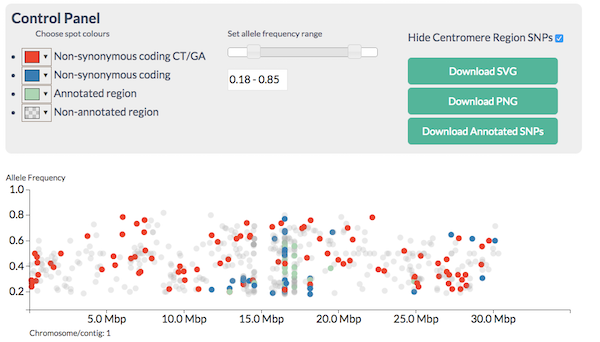
\includegraphics[width=4in]{assets/candisnp} \caption{Screenshot of the CandiSNP tool. Spots represent SNPs
(height on the \texttt{y} axis shows major allele frequency).}\label{fig:csnpb4}
\end{figure}

CandiSNP allows you to look at the SNPs like in Figure \ref{fig:csnpb4}
and apply filters to narrow down the region and candidates so you see
something like Figure \ref{fig:csnp}. CandiSNP takes a VCF file as
input.




\begin{figure}
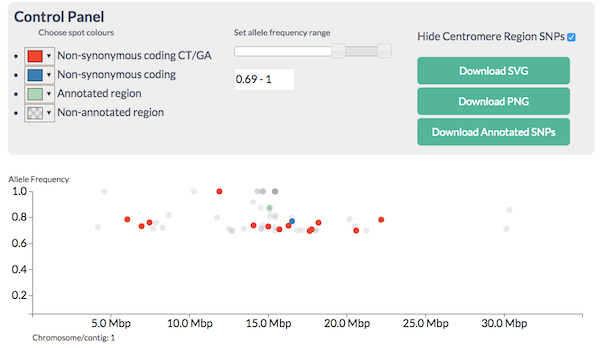
\includegraphics[width=4in]{assets/candisnp_after} \caption{CandiSNP after filtering. The region of the high red
spot density is the recombinant region}\label{fig:csnp}
\end{figure}

\section{Density plots}\label{density-plots}

Statistical methods are useful when the number of SNPs generated is so
large that you can't visualise them all at the same time. Density plots
like Figure \ref{fig:densityp} (which is of the same data as the
CandiSNP plot in \ref{fig:csnpb4} help us to see the rough patterns in a
similar way. The homozygous and heterozygous show an increase in the
SNP-rich centromeric region which biases the data and an overall
decrease at the far right of the chromosome, but the enriched region is
visible in the high ratio at about 17Mbp as in the CandiSNP output.
These kinds of plots can be generated with Galaxy's plotting tools.




\begin{figure}
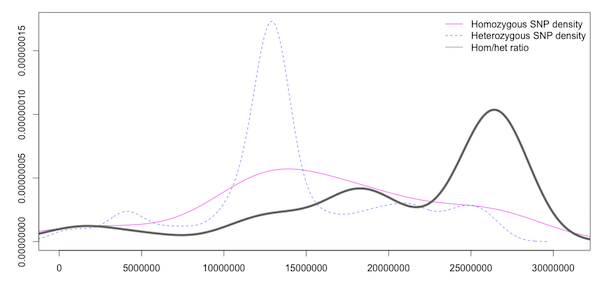
\includegraphics[width=4in]{assets/density} \caption{Density plot of homozygous, heterozygous SNP density and
the ratio of hom/het SNPS in sliding windows}\label{fig:densityp}
\end{figure}

\section{Centromeres}\label{centromeres}

Centromeres are a real problem with these sorts of analysis. They are so
SNP rich that they swamp analysis and visualisations. It helps to just
screen them out from the analysis. CandiSNP will let you turn off
centromeres associated SNPs, Galaxy tools can also help you filter them
out.

\section{SNP Deletion - Fewer are
better}\label{snp-deletion---fewer-are-better}

Perhaps it is counter-intuitive but getting fewer SNPs is often better
in these approaches. A common source of confounding SNPs is from the
parental line itself. All individuals of any species have differences in
the genomes from the references we use to call SNPs, and some (perhaps
many) of these will be shared between the parent used to generate the
mutants and the mutants. By sequencing the parent line and calling SNPs
between it and the reference genome, you get a list of parental SNPs
that you can often delete straight out of the mutant as being
non-causative.

\section{Exercises}\label{exercises-3}

\subsection{Analyse SNP data with
CandiSNP}\label{analyse-snp-data-with-candisnp}

You have some whole genome \emph{Arabidopsis} SNP data annotated with
SNPEff in the shared data library \texttt{Annotation}, the VCF file
\texttt{filtered\_snps.vcf}. Use this in the web version of CandiSNP
tool at {[}{]} This data set is a real one and we know exactly where the
mutation is because we've sequenced it, so there is a \emph{right}
answer. Use the sliders and filter tools to find a region enriched in
homozygous candidate SNPs.

Please complete the questions at
\url{https://goo.gl/forms/KnqB9IdRXRB3rQbu1}

\begin{enumerate}
\def\labelenumi{\arabic{enumi}.}
\tightlist
\item
  Can you come up with candidate regions / genes for the causative
  mutation?
\item
  Which is more useful, filtering or colouring?
\item
  How much extra information does knowing the genes the SNPs fall in
  give? Especially in a case where you might know something about the
  biology already.
\end{enumerate}

\subsection{Generate density plots of different SNP
classes}\label{generate-density-plots-of-different-snp-classes}

Standard Galaxy tools can generate histograms of data. However the data
needs to be in tabular format, not VCF. Here's a little recipe for going
from VCF to a table that is useful.

\begin{enumerate}
\def\labelenumi{\arabic{enumi}.}
\tightlist
\item
  To make a tabular file, use the
  \texttt{Text\ Manipulation\ ..\ Cut\ Columns\ Tool}. Cut out columns
  \texttt{c1,c2,c3,c4,c8,c9}.
\item
  To strip text from the AF field and just leave the numbers, use the
  \texttt{Text\ Manipulation\ ..\ Trim\ Leading} on \texttt{column\ 5},
  trim to position \texttt{4} and set to \texttt{ignore} \texttt{\#}.
\item
  To get the homozygous SNPs, use the
  \texttt{Filter\ and\ Sort\ ..\ Filter\ data\ on\ any\ column} tool.
  Filter on \texttt{c5\textgreater{}=0.75} (or whatever seems sensible
  to you).
\item
  To get the heterozygous SNPs, do step \texttt{3} again but filter on
  \texttt{c5\textless{}0.75}.
\end{enumerate}

This will leave you with two files on which to carry out the remaining
steps.

\begin{enumerate}
\def\labelenumi{\arabic{enumi}.}
\setcounter{enumi}{4}
\tightlist
\item
  To split the files into single chromosome files use
  \texttt{Text\ Manipulation\ ..\ Split\ file\ according\ to\ value\ of\ a\ column}
  use \texttt{column\ 1} (the chromosome column)
\item
  For each resulting file you can use \texttt{Plotting\ ..\ Histogram}
  to make the histograms. It is useful to add the density plot and to
  use around 150 breaks.
\end{enumerate}

With a bit more work you can combine the different plots into one large
one for easier comparison, and you can use sliding window tools to
calculate the ratio of Hom/Het SNPs across the chromosomes.

\subsection{Comparing density plots}\label{comparing-density-plots}

\begin{enumerate}
\def\labelenumi{\arabic{enumi}.}
\tightlist
\item
  Use the numerous density plots you made to compare the likely
  positions of the causative SNPs
\item
  Can you narrow down the area sufficiently to examine the text list in
  more detail?
\item
  What further filtering could you do to make the plots more effective?
\end{enumerate}

\bibliography{refs.bib}


\end{document}
